\documentclass{article}

\usepackage[hidelinks]{hyperref}
\usepackage{graphicx}
\graphicspath{ {images/} }
\usepackage[margin=1in, includefoot]{geometry}
\usepackage{tikz}  
\usepackage{fancyvrb}
\usetikzlibrary{decorations.markings}
\pgfdeclarelayer{bg}    % declare background layer
\pgfsetlayers{bg,main}
\usepackage{amsmath}
\usepackage{todonotes}
\usepackage[utf8]{inputenc}

% header and footer 
\usepackage{fancyhdr}
\pagestyle{fancy}
\fancyhead{}
\fancyfoot{}
\fancyfoot[R]{\thepage}
\renewcommand{\headrulewidth}{0pt}
\renewcommand{\footrulewidth}{0pt}

\begin{document}
\begin{titlepage}

	\begin{center}
	
	\huge{\bfseries Advanced Algorithm Assignment}\\
	[1cm]
	\line(1,0){350}\\
	[0.15in]
	\textit{\huge{\bfseries{ Implement Dijkstra algorithm using Fibonacci heap}}}\\
	\line(1,0){200}\\
	[1cm]
	\textrm{\bfseries{\LARGE Team Finite}}\\
	[1cm]
	\textrm{\bfseries{\LARGE IIT Indore}}\\
	[8.2cm]
	\end{center}
	\begin{minipage}{0.25\linewidth}
	\begin{flushright}
	\textrm{\large
	{\bfseries Submitted to :}
	\\Dr.Ranveer Singh
	\\Assistant Professor
	\\Department of Computer Science
	\\IIT Indore
	}
	\end{flushright}
	\end{minipage}
	\hfill
	\begin{minipage}{0.25\linewidth}
	\begin{flushleft}
	\textrm{\large
	{\bfseries Team Members:}
	\\ Ananya Roy 
	\\Atharva Tendulkar
	\\K Bharath
	\\Mohit Kumar
	\\Shibani Das}
	\end{flushleft}
	\end{minipage}

\end{titlepage}

\tableofcontents
\thispagestyle{empty}
\cleardoublepage
\setcounter{page}{1}

\section*{Problem Statement: Implement Dijkstra algorithm using Fibonacci heap on the given graph.}\label{sec:spanning}
\section{Dijkstra’s Algorithm }
\begin{enumerate}
\item Dijkstra's Algorithm is used to find the shortest route from one vertex, called the source, to all others in a weighted graph, but it can be adapted to focus the distance to one node, called a target.
\item Dijkstra's algorithm makes use of weights of the edges for finding the path that minimizes the total distance (weight) among the source node and all other nodes. This algorithm is also known as the single-source shortest path algorithm.
\item Dijkstra’s algorithm is the iterative algorithmic process to provide us with the shortest path from one specific starting node to all other nodes of a graph.
\item It is important to note that Dijkstra’s algorithm is only applicable when all weights are positive because, during the execution, the weights of the edges are added to find the shortest path.
\item Generally, Dijkstra’s algorithm works on the principle of relaxation where an approximation of the accurate distance is steadily displaced by more suitable values until the shortest distance is achieved.
\item Also, the estimated distance to every node is always an overvalue of the true distance and is generally substituted by the least of its previous value with the distance of a recently determined path. 
\item It uses a priority queue to greedily choose the nearest node that has not been visited yet and executes the relaxation process on all of its edges.
\end{enumerate}

\section{Fibonacci Heap}
Fibonacci Heap is a collection of trees with min-heap or max-heap property. In Fibonacci Heap, trees can have any shape even all trees can be single nodes (This is unlike Binomial Heap where every tree has to be Binomial Tree). It is used for priority queue operations, consisting of a collection of heap-ordered trees. It has a better amortized running time than many other priority queue data structures including the binary heap and binomial heap.
\subsection{Properties}
\begin{enumerate}
\item Set of heap-ordered trees. 
\item Maintain pointer to minimum element.
\item Set of marked nodes which are used to keep the heaps flat.
\item The trees within a Fibonacci heap are unordered but rooted.
\end{enumerate}

Below is the diagram of a Fibonacci heap.

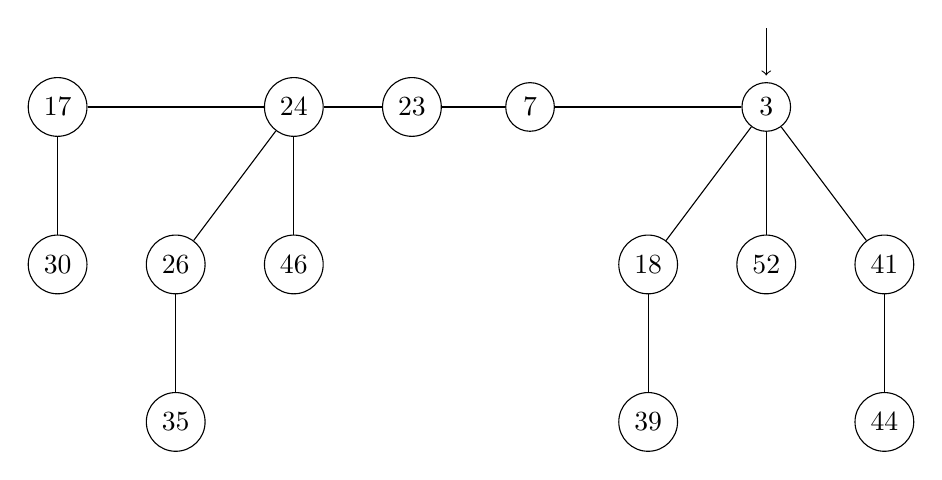
\begin{tikzpicture}  
  [scale=1,auto=center, every node/.style={circle,draw=black!100}] % here, node/.style is the style pre-defined, that will be the default layout of all the nodes. You can also create different forms for different nodes.  
    
  \node (a1) at (2,4.5) {17};  
  \node (a2) at (5,4.5)  {24};
  \node (a3) at (6.5,4.5)  {23};  
  \node (a4) at (8,4.5) {7};
  \node (a5) at (11,4.5) {3};  
  \node (a6) at (2,2.5)  {30};  
  \node (a7) at (3.5,2.5)  {26};  
  \node (a8) at (5,2.5) {46};
  \node (a9) at (9.5,2.5) {18};
  \node(a10) at (11,2.5) {52};
  \node(a11) at (12.5,2.5) {41};
  \node(a12) at (3.5,0.5) {35};
  \node(a13) at (9.5,0.5) {39};
  \node(a14) at (12.5,0.5) {44};
  
  
  \draw(a1) -- (a2); 
  \draw(a2) -- (a3);
  \draw(a3) -- (a4);
  \draw(a4) -- (a5);
  \draw(a1) -- (a6);
  \draw(a2) -- (a7);
  \draw(a2) -- (a8);
  \draw(a5) -- (a9);
  \draw(a5) -- (a10);
  \draw(a5) -- (a11);
  \draw(a7) -- (a12);
  \draw(a9) -- (a13);
  \draw(a11) -- (a14);
  
  \draw[->] (11,5.5) -- (11,4.9);
  
\end{tikzpicture}
\newline
\textbf{Figure 1: Fibonacci heap}
\newline
\newline

\section{Code Section}
\subsection{Pseudo Code}
 \begin{verbatim}
singleSourceShortest(G,s)
1. PQ = new Priority Queue
2. foreach v in V do 
3. 		dist[v] = infi
4. 		pred[v] = -1
5. dist[s] = 0
6. foreach v in V do
7.		insert(v,dist[v]) into PQ

8. While(PQ is not empty) do
9.   u = getMin(PQ)
10.  foreach neighbor v of u do
11.    w = weight of edge(u,v)
12.    newLen = dist[u] + w
13.    if(newLen < dist[v]) then
14.        decreaseKey(PQ,v,newLen)
15.        dist[v]=newLen   
 
 \end{verbatim}
\subsection{Code Repository}
Code implementation in C++ language can be found following hyperlink :  \href{https://github.com/mohit83k/iiti_ms_assignments/blob/main/advancedalgo/4-5/dijkstra.cpp}{Assignment 4-5 cpp code}.
\subsection{Explanation}
\begin{enumerate}
\item Create an empty Fibonacci Heap (line 1)
\item	Assign to every vertex a tentative distance value: set it to zero for our source vertex and to infinity for all other vertices. Set the source vertex as current (line 2 to 5).
\item	Insert all (v, dist [v]) in Fibonacci heap (line 6 and 7)
\item	select the unvisited vertex (vertex that is still in Heap) that is marked with the smallest tentative distance, set it as the new "current vertex” and remove it from Fibonacci heap (line 9)
\item	For the current vertex, consider all of its unvisited neighbours and calculate their tentative distances through the current vertex by adding the weight of the edge connecting the current vertex and neighbour to the current vertex's assigned value. Compare the newly calculated tentative distance to the current assigned value and assign the smaller one. (Line 10 - 16)
\item	Once Fibonacci heap is empty, then stop. (Line 8)
\item	Otherwise, and continue while loop (Line 4 onwards). 

\end{enumerate}

\section{Complexity Analysis}
\begin{enumerate}
\item	Normal Dijkstra’s algorithm which is implemented using simple arrays can run in O(n$^{2}$) time
\item	Dijkstra's algorithm can be implemented more efficiently by storing the graph in the form of adjacency lists and using a Fibonacci heap as a priority queue to implement extracting minimum efficiently. 
\item	Fibonacci heaps are sometimes referred to as “lazy” data structures because their structure is less strictly managed as they perform operations than in many other data structures. But this “laziness” allows them to have extremely fast amortized time complexities for common heap operations.
\item	Following are complexities of Fibonacci heap\\\\
\begin{tabular}{ll}
Operation		&	TimeComplexity\\\\
insert()	&		O(1)\\
reportMin()	&		O(1)\\
deleteMin()	&		O(log(n)) amortized\\
decreaseKey()	&	O(1) amortized\\
merge()		&		O(1)\\
\end{tabular}
\item Line 8 says that, we will execute until heap is empty i.e. we visit all the nodes. So, from this we can say that our outer loop will run O(V) times
\item	From pseudo code, we can say that
T(n) = O (V * (pop vertex from min heap + find unvisited vertices in edges * push them to min heap)) 
{i.e., for Outer loop which runs V times we need to do :$\rightarrow$ (pop vertex from min heap + find unvisited vertices in edges * push them to min heap)}
\item	Hence, T(n) =   O (V * (pop vertex from min heap + E * push unvisited vertices to min heap)). 
Note, that we can push the same node multiple times here before we get to "visit" it.
\item	T(n) = O (V * (log (heap size) + E * log (1)))
\item	Hence T(n) = O (V * (log(V) + E))
\item	Hence, T(n) = O (V log V + VE)
\item	But, E = V because each vertex can reference all other vertices
\item	Hence, T(n) = O (V log V + V$^{2}$)
\item	V$^{2}$ is also a total number of edges, so if we let E = V$^{2}$ (as in the official naming), we will T(n) = O (V log V + E)


\end{enumerate}

\end{document}